\documentclass[11pt]{article}
\usepackage[utf8]{inputenc}
\usepackage{graphicx}
\usepackage[width = 6.5 in, height = 9 in]{geometry}
\usepackage{listings}

\begin{document}

\begin{center}
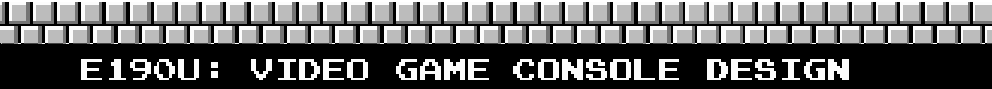
\includegraphics[width=\textwidth]{title}

\textbf{E190U:} Lab 6 - Motion Capture Pong\\
Lab Draft by Amy Ngai\\
Spring 2015


\includegraphics[width=\textwidth]{bottom}
\end{center}


\section{Requirement}
Incorporate hand motion capture into the provided game of Pong. After you have accomplished this task, please incorporate on additional asset of motion detection into a game. Specific integration of motion detection input in other games is up to the discretion of the student. However, the game is expected to be reasonable and playable.  There are minimal requirements for this lab so you are strongly encouraged to be creative and go further than the minimum requirements. As with the previous lab, the system is not expected to be entirely robust, but should be reliable and return expected and repeatable results.

\section{Discussion}
You will be provided code for a generic game of pong in PyGame that takes in standard keyboard input. The code for the game relies on PyGame which needs
to be installed on the board. To install Pygame, simply run this command in terminal:
\begin{lstlisting}
	sudo apt-get install python-pygame
\end{lstlisting}
As a start, you can incorporate motion capture into this game of pong by governing the paddle position with the detected hand position. This can be done by extracting the part of the PyGame code that affects the paddle position and extracting the hand motion from your motion detection code and integrating these two components. An important consideration is the limitations of motion capture. Consider edge cases where the hand is literally at the edge of the screen. Consider the range at which detection is most accurate. Make sure to incorporate these limitations  in your motion capture design. \\ \\

Beyond the required implementation, creativity is strongly encouraged in this lab (as with all the others) to go further. We are requiring you to do another incorporation of motion capture into a game, but we are leaving the actual design open ended. Consider different objects, different effects, different games... Really, go crazy!
\end{document}
